\documentclass[border=6pt]{standalone}
\usepackage{amsmath,amssymb,bm}
\newcommand{\bL}{\mathbf{L}}
\usepackage{tikz}
\usetikzlibrary{arrows.meta,decorations.pathmorphing,positioning}
\definecolor{cRaise}{HTML}{0072B2}
\definecolor{cLower}{HTML}{D55E00}
\definecolor{cKeep}{HTML}{009E73}
\definecolor{cKill}{HTML}{D55E00}
\begin{document}
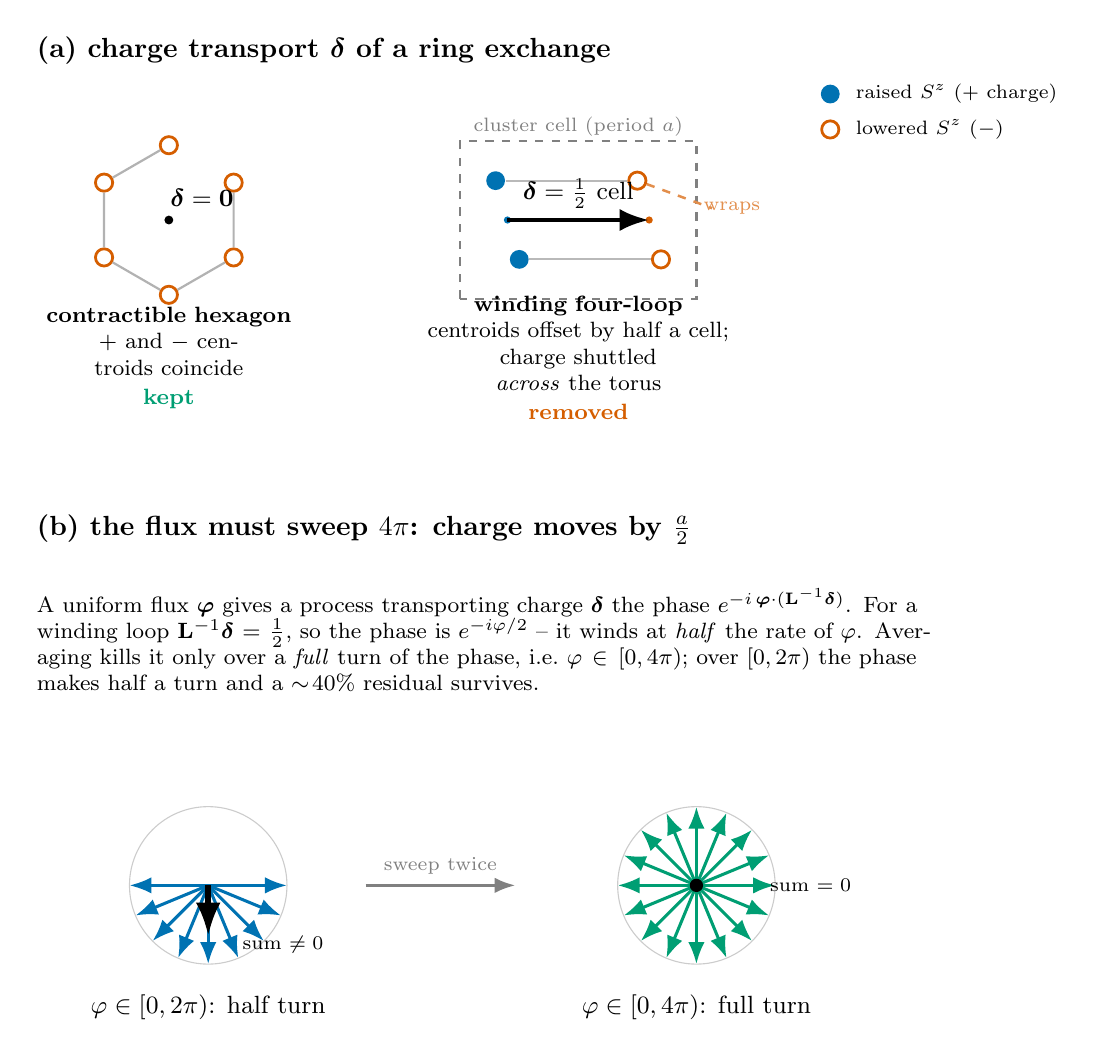
\begin{tikzpicture}[
  raise/.style={circle,fill=cRaise,inner sep=2.4pt},
  lower/.style={circle,draw=cLower,line width=1pt,fill=white,inner sep=2.2pt},
  >=Latex]

%============================ PANEL A: what delta is ============================
\node[anchor=south west,font=\bfseries] at (-0.3,3.4)
  {(a) charge transport $\bm\delta$ of a ring exchange};

% --- contractible hexagon: raised/lowered balanced, delta=0 ---
\begin{scope}[shift={(1.5,1.55)}]
  \foreach \a/\ty in {90/r,150/l,210/r,270/l,330/r,30/l}
    \node[\ifx\ty r raise\else lower\fi] (h\a) at (\a:0.95) {};
  \draw[gray!60,line width=0.8pt] (h90)--(h150)--(h210)--(h270)--(h330)--(h30)--cycle;
  \fill[black] (0,0) circle (1.6pt);
  \node[font=\small] at (0.42,0.28) {$\bm\delta=\bm0$};
  \node[font=\footnotesize,text width=3.2cm,align=center] at (0,-1.75)
    {\textbf{contractible hexagon}\\ $+$ and $-$ centroids coincide\\[1pt]
     \textcolor{cKeep}{\textbf{kept}}};
\end{scope}

% --- winding 4-loop: raised/lowered offset by half a cell, delta = a/2 ---
\begin{scope}[shift={(6.7,1.55)}]
  \draw[gray,dashed,line width=0.8pt] (-1.5,-1.0) rectangle (1.5,1.0);
  \node[gray,font=\scriptsize] at (0,1.18) {cluster cell (period $a$)};
  \node[raise] (a) at (-1.05,0.5) {};
  \node[raise] (c) at (-0.75,-0.5){};
  \node[lower] (b) at (0.75,0.5) {};
  \node[lower] (d) at (1.05,-0.5){};
  \draw[gray!55,line width=0.8pt] (a)--(b) (c)--(d);
  \draw[cLower!70,line width=0.9pt,dashed] (b)--(1.7,0.15);
  \node[cLower!70,font=\scriptsize] at (1.95,0.15) {wraps};
  \coordinate (cp) at (-0.9,0.0);
  \coordinate (cm) at (0.9,0.0);
  \fill[cRaise] (cp) circle (1.3pt); \fill[cLower] (cm) circle (1.3pt);
  \draw[->,line width=1.7pt,black] (cp)--(cm)
       node[midway,above,font=\small] {$\bm\delta=\tfrac12$ cell};
  \node[font=\footnotesize,text width=3.9cm,align=center] at (0,-1.75)
    {\textbf{winding four-loop}\\ centroids offset by half a cell;\\
     charge shuttled \emph{across} the torus\\[1pt]
     \textcolor{cKill}{\textbf{removed}}};
\end{scope}

% legend
\node[raise] at (9.9,3.15) {}; \node[anchor=west,font=\scriptsize] at (10.1,3.15) {raised $S^z$ ($+$ charge)};
\node[lower] at (9.9,2.7) {};  \node[anchor=west,font=\scriptsize] at (10.1,2.7) {lowered $S^z$ ($-$)};

%============================ PANEL B: why 4pi ============================
\begin{scope}[shift={(0,-6.2)}]
\node[anchor=south west,font=\bfseries] at (-0.3,3.5)
  {(b) the flux must sweep $4\pi$: charge moves by $\tfrac{a}{2}$};
\node[anchor=north west,font=\footnotesize,text width=11.5cm] at (-0.3,3.2)
  {A uniform flux $\bm\varphi$ gives a process transporting charge $\bm\delta$ the phase
   $e^{-i\,\bm\varphi\cdot(\bL^{-1}\bm\delta)}$. For a winding loop
   $\bL^{-1}\bm\delta=\tfrac12$, so the phase is $e^{-i\varphi/2}$ -- it winds at
   \emph{half} the rate of $\varphi$. Averaging kills it only over a \emph{full} turn of the phase,
   i.e.\ $\varphi\in[0,4\pi)$; over $[0,2\pi)$ the phase makes half a turn and a $\sim\!40\%$ residual survives.};

% phasor [0,2pi): angles 0..-pi (half circle) sum != 0
\begin{scope}[shift={(2.0,-0.7)}]
  \draw[gray!40] (0,0) circle (1.0);
  \foreach \k in {0,...,8}{
    \pgfmathsetmacro\ang{-\k*180/8}
    \draw[cRaise,line width=1.1pt,->] (0,0)--(\ang:1.0);
  }
  \draw[black,line width=2pt,->] (0,0)--(-90:0.64);
  \node[font=\scriptsize] at (0.95,-0.75){sum $\neq 0$};
  \node[font=\small] at (0,-1.55) {$\varphi\in[0,2\pi)$: half turn};
\end{scope}

% phasor [0,4pi): full circle sum = 0
\begin{scope}[shift={(8.2,-0.7)}]
  \draw[gray!40] (0,0) circle (1.0);
  \foreach \k in {0,...,15}{
    \pgfmathsetmacro\ang{-\k*360/16}
    \draw[cKeep,line width=1.1pt,->] (0,0)--(\ang:1.0);
  }
  \fill[black] (0,0) circle (2.4pt);
  \node[font=\scriptsize] at (1.45,0.0){sum $=0$};
  \node[font=\small] at (0,-1.55) {$\varphi\in[0,4\pi)$: full turn};
\end{scope}
\draw[->,gray,line width=1pt] (4.0,-0.7)--(5.9,-0.7) node[midway,above,font=\scriptsize]{sweep twice};
\end{scope}

\end{tikzpicture}
\end{document}
